% Standalone influence diagram of the routing MDP: states in a row, decisions below,
% the stroke subtype a hidden component of S_0 revealed at S_1, one terminal reward.
%   pdflatex fig_influence_standalone.tex
% Colors match viz/paper_figures.jl (blue / orange / teal).
\documentclass[tikz, border=6pt]{standalone}
\usepackage[T1]{fontenc}
\usepackage{mathptmx}
\usepackage{amsmath}
\usetikzlibrary{arrows.meta, shapes.geometric, calc}
\definecolor{pblue}{RGB}{42,120,214}
\definecolor{porange}{RGB}{235,104,52}
\definecolor{pteal}{RGB}{27,175,122}

\begin{document}
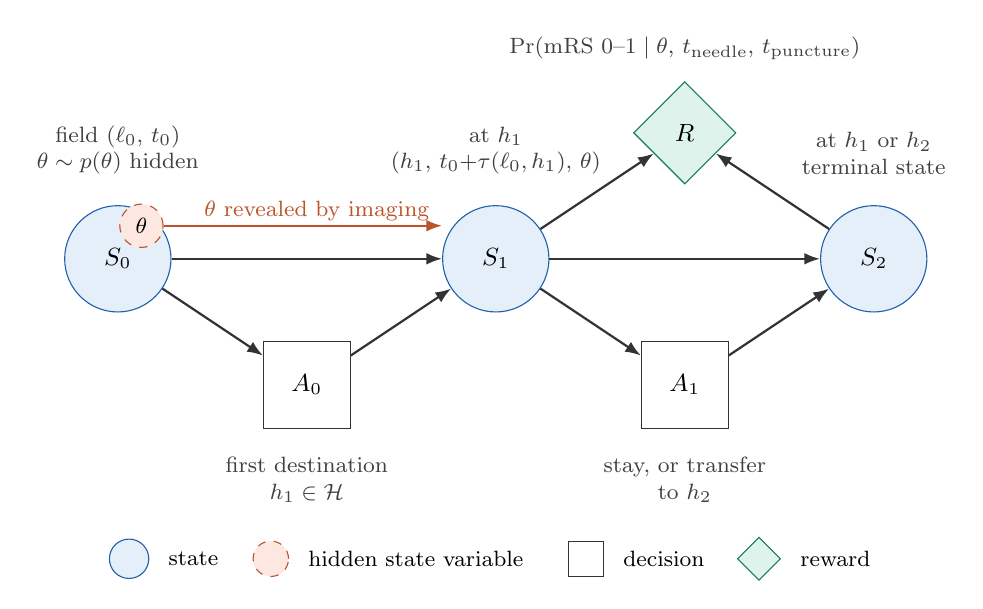
\begin{tikzpicture}[
  font=\small, >={Latex[length=2mm]},
  state/.style ={circle, fill=pblue!12, draw=pblue!80!black, minimum size=1.35cm, inner sep=1pt},
  hidden/.style={circle, fill=porange!15, draw=porange!80!black, dashed, minimum size=0.55cm, inner sep=0pt, font=\footnotesize},
  action/.style={rectangle, draw=black!80, fill=white, minimum size=1.1cm, inner sep=2pt},
  reward/.style={diamond, fill=pteal!15, draw=pteal!70!black, minimum size=1.3cm, inner sep=0pt, aspect=1.2},
  lab/.style={font=\footnotesize, align=center, text=black!75},
  edge/.style={->, thick, black!80},
  reveal/.style={->, thick, porange!80!black},
]

% ---- nodes: states on one line, decisions below, reward above
\node[state]  (s0) at (0,0)   {$S_0$};
\node[state]  (s1) at (4.8,0) {$S_1$};
\node[state]  (s2) at (9.6,0) {$S_2$};
\node[hidden] (th) at ($(s0.center)+(0.3,0.42)$) {$\theta$};
\node[action] (a0) at (2.4,-1.6) {$A_0$};
\node[action] (a1) at (7.2,-1.6) {$A_1$};
\node[reward] (r)  at (7.2,1.6)  {$R$};

% ---- edges (all straight)
\draw[edge] (s0) -- (s1);
\draw[edge] (s1) -- (s2);
\draw[edge] (s0) -- (a0);
\draw[edge] (a0) -- (s1);
\draw[edge] (s1) -- (a1);
\draw[edge] (a1) -- (s2);
\draw[edge] (s1) -- (r);
\draw[edge] (s2) -- (r);
\draw[reveal] (th.east) -- node[above, pos=0.55, inner sep=1.5pt, font=\footnotesize, text=porange!80!black] {$\theta$ revealed by imaging} ($(s1.west)+(0,0.42)$);

% ---- labels
\node[lab, anchor=south] at ($(s0.center)+(0,0.95)$) {field $(\ell_0,\, t_0)$\\ $\theta \sim p(\theta)$ hidden};
\node[lab, anchor=south] at ($(s1.center)+(0,0.95)$) {at $h_1$\\ $(h_1,\, t_0{+}\tau(\ell_0,h_1),\, \theta)$};
\node[lab, anchor=south] at ($(s2.center)+(0,0.95)$) {at $h_1$ or $h_2$\\ terminal state};
\node[lab, anchor=north] at ($(a0.center)+(0,-0.8)$) {first destination\\ $h_1 \in \mathcal{H}$};
\node[lab, anchor=north] at ($(a1.center)+(0,-0.8)$) {stay, or transfer\\ to $h_2$};
\node[lab, anchor=south]  at ($(r.north)+(0,0.15)$) {$\Pr(\text{mRS } 0\text{--}1 \mid \theta,\, t_{\text{needle}},\, t_{\text{puncture}})$};

% ---- legend, centred under the diagram
\coordinate (lc) at ($(current bounding box.south)+(0,-0.6)$);
\begin{scope}[font=\footnotesize]
  \node[state,  minimum size=0.5cm]  (l1) at ($(lc)+(-4.6,0)$) {};
  \node[anchor=west] at ($(l1.east)+(0.12,0)$) {state};
  \node[hidden, minimum size=0.45cm] (l2) at ($(lc)+(-2.8,0)$) {};
  \node[anchor=west] at ($(l2.east)+(0.12,0)$) {hidden state variable};
  \node[action, minimum size=0.45cm] (l3) at ($(lc)+(1.2,0)$) {};
  \node[anchor=west] at ($(l3.east)+(0.12,0)$) {decision};
  \node[reward, minimum size=0.55cm] (l4) at ($(lc)+(3.4,0)$) {};
  \node[anchor=west] at ($(l4.east)+(0.12,0)$) {reward};
\end{scope}

\end{tikzpicture}
\end{document}
